\vspace{0.5cm}


\section*{Problema 3.45}
Para la trayectoria Adiabática Húmeda desde el punto $1000hPa$ y $25^o C$, hasta una altura de $250hPa$ se tiene una temperatura de $-35.5^o C$ y al aumentar un grado, se llega a una temperatura de $-33.5^o C$. Con lo que la diferencia es de $\boxed{\sim 2^o C}$
	
\section*{Problema 3.48}




%\section*{Anexo}
%\begin{figure}[H]
%	\centering
%	 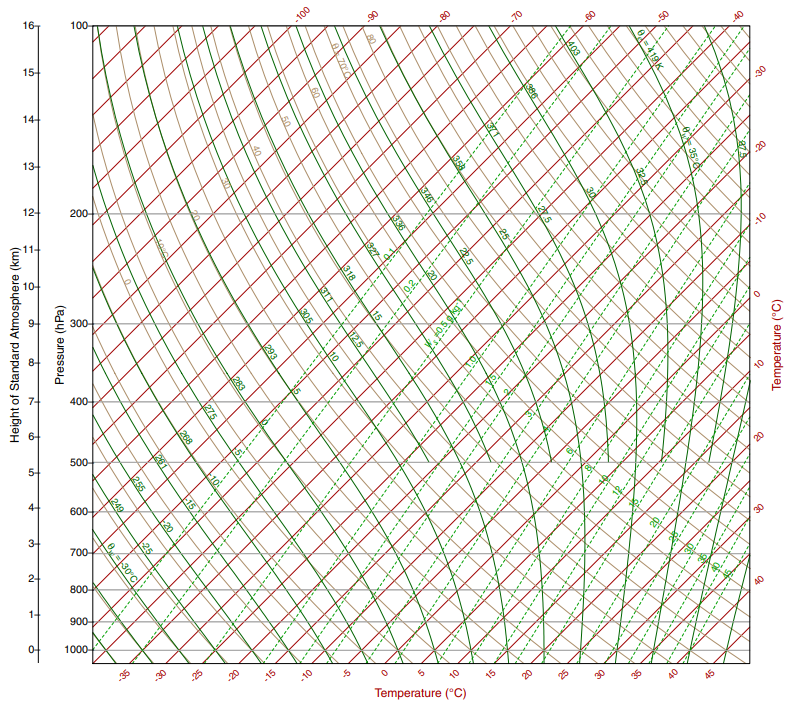
\includegraphics[scale=0.7]{./img/skewTlnp.png}
%	 \caption{Skew $T-\ln{p}$ Chart, book website.}
%	 \label{skew}
%\end{figure}



















%%%%%